% Asset ID: AS1CoordinateGeometryCirclesTikZ-001
% Source: Chapter 6 Circles evidence, chord and perpendicular bisector
% Purpose: Show a chord, its midpoint, and its perpendicular bisector passing through the centre.
\documentclass[tikz,border=8pt]{standalone}
\usetikzlibrary{calc,angles,quotes}
\begin{document}
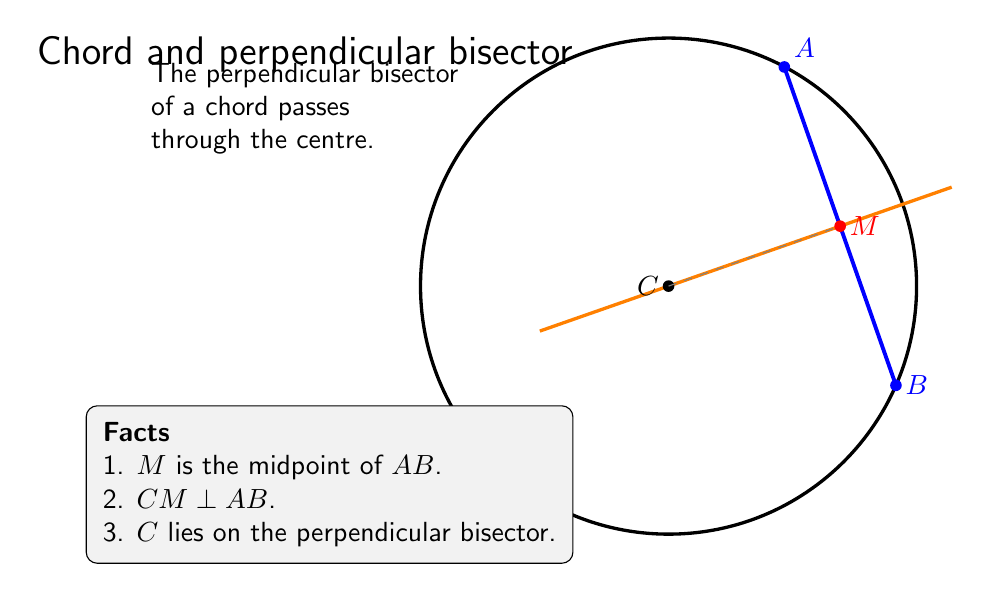
\begin{tikzpicture}[scale=1.05, font=\sffamily]
\coordinate (C) at (0,0); \draw[line width=1.2pt] (C) circle (3);
\coordinate (A) at (1.4,2.65); \coordinate (B) at (2.75,-1.2); \coordinate (M) at ($(A)!0.5!(B)$);
\draw[line width=1.4pt, blue] (A) -- (B); \fill[blue] (A) circle (2pt) node[above right] {$A$}; \fill[blue] (B) circle (2pt) node[right] {$B$};
\draw[line width=1.2pt, orange] ($(C)!-0.75!(M)$) -- ($(C)!1.65!(M)$);
\fill[black] (C) circle (2pt) node[left] {$C$}; \fill[red] (M) circle (2pt) node[right] {$M$}; \draw[dashed, gray] (C) -- (M);
\node[align=center] at (-4.4,2.8) {\Large Chord and perpendicular bisector};
\node[align=left] at (-4.4,2.15) {The perpendicular bisector\\of a chord passes\\through the centre.};
\node[align=left, draw, rounded corners, fill=gray!10, inner sep=6pt] at (-4.1,-2.4) {\textbf{Facts}\\1. $M$ is the midpoint of $AB$.\\2. $CM \perp AB$.\\3. $C$ lies on the perpendicular bisector.};
\end{tikzpicture}\end{document}
